\documentclass{article}
\usepackage{tikz}
\usetikzlibrary{arrows.meta,positioning,calc,shapes.geometric}
\pagestyle{empty}
\begin{document}
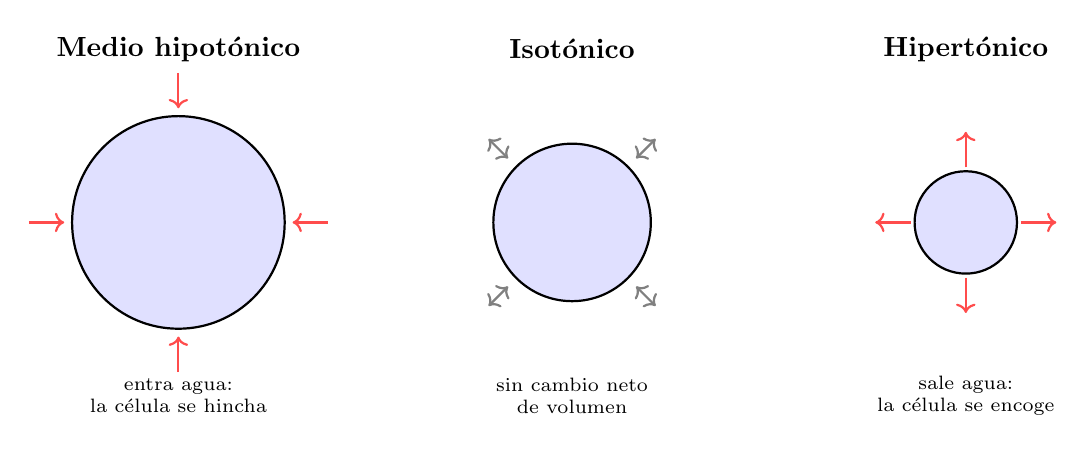
\begin{tikzpicture}
\tikzset{every node/.append style={align=center}}

\def\cell#1#2#3{\draw[thick, fill=#3] (#1,0) circle (#2);}
\cell{0}{1.35}{blue!12}\cell{5}{1.0}{blue!12}\cell{10}{0.65}{blue!12}
\node[font=\bfseries] at (0,2.2) {Medio hipotónico}; \node[font=\bfseries] at (5,2.2) {Isotónico}; \node[font=\bfseries] at (10,2.2) {Hipertónico};
\node[font=\scriptsize, align=center] at (0,-2.2) {entra agua:\\ la célula se hincha}; \node[font=\scriptsize, align=center] at (5,-2.2) {sin cambio neto\\ de volumen}; \node[font=\scriptsize, align=center] at (10,-2.2) {sale agua:\\ la célula se encoge};
\foreach \a in {0,90,180,270} {\draw[->, thick, red!70] (0,0)+(\a:1.9) -- +(\a:1.45);}
\foreach \a in {45,135,225,315} {\draw[<->, thick, gray] (5,0)+(\a:1.5) -- +(\a:1.15);}
\foreach \a in {0,90,180,270} {\draw[->, thick, red!70] (10,0)+(\a:0.7) -- +(\a:1.15);}

\end{tikzpicture}
\end{document}
